\section{Outlook and Conclusions}
\begin{figure}[htb]
    \centering
    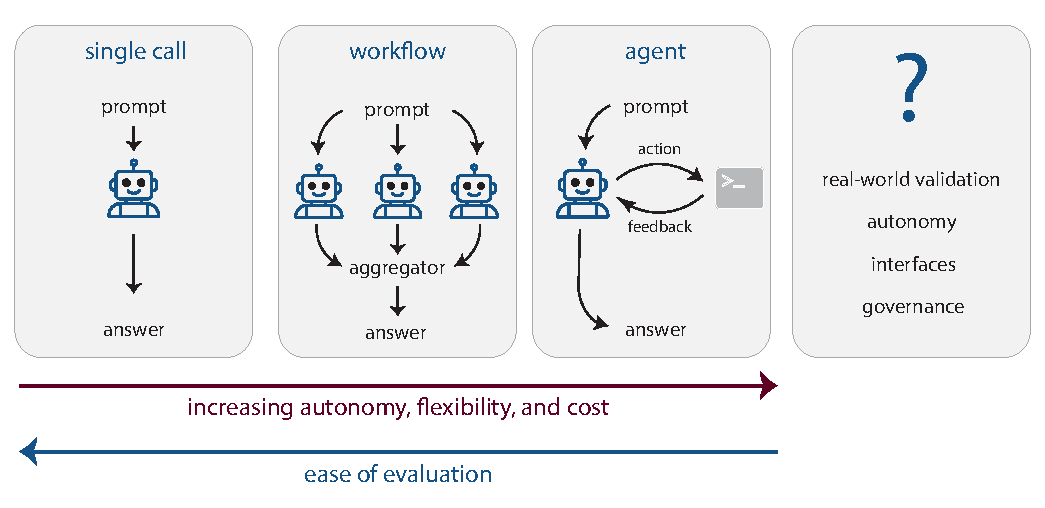
\includegraphics[width=1\linewidth]{figures/conclusion_figure_v2.pdf}
    \caption{\textbf{Evolution of \gls{gpm}-powered systems.} First \gls{gpm} applications directly used zero- or few-shot prompted or fine-tuned \glspl{gpm}. More complex tasks could be solved by combining multiple \glspl{gpm} in workflows where the execution trajectory is pre-determined. In agents, \glspl{gpm} autonomously decide on the execution trajectory and in this way enable researchers to address open-ended tasks. Moving forward, coupling the validation closer to real-world objectives with further increased validation in better, custom user interfaces will enhance the impact of \glspl{gpm}. To ensure safe and ethical deployment, the community must engage with the broader public and policymakers to devise governance strategies.}
    \label{fig:conclusions}
\end{figure}

As we have explored in this review, \glspl{gpm}---especially \glspl{llm}---hold remarkable promise for the chemical sciences. 
The field moved from using models in simple single calls to a \glspl{gpm} to developing workflows, in which a sequence of calls is performed, to increasingly complex autonomous agents in which the model decides on its own trajectory (see \Cref{fig:conclusions}). To power those agents, increasingly powerful models are being built, including reasoning models that promise higher data efficiency. 

Yet, several fundamental questions remain unresolved. We do not understand if there are fundamental limits to what can be predicted, given the inherent unpredictability of chemical systems and the reliance on tacit knowledge. We do not know what new datasets and techniques need to be developed, given the fact that the knowledge we extract from already published data is approaching a limit.\autocite{silver2025welcome} New data most likely will be generated by agents learning from their own experience.
To optimize systems, we need to better understand the underlying structure of chemical data.
In many other fields, data distributions have been shaped by special driving forces. 
For example, evolution led to a direct link between sequence and fitness in biological sequences, which makes such datasets special. In chemistry it is unclear what the \enquote{driving force} that shapes datasets is. 

It is also unclear how quickly these innovations will permeate the average chemistry lab, where the adoption of new technology depends on more than just predictive prowess. 
And we also do not know yet how we should interface with those models for the greatest effectiveness.
In addition, it is also unclear how far acceleration can take us, as nature imposes some natural speed limits: Some experiments simply take their time. 

Overall, this landscape suggests a future rich with opportunity. But realizing the potential impact of \glspl{gpm} demands clear-eyed caution: while it is now deceptively easy to spin up prototypes, transforming them into robust, reliable tools is a far more arduous task. \autocite{sculley2014machine}
More crucial still is our need for rigorous measurement and feedback---whether in the construction of evaluation suites, the calibration of reward functions for reinforcement learning, or the design of sensible governance. 
No single discipline can shoulder this alone; chemists, policy experts, and computer scientists must broaden their ranks and collaborate. 
This is particularly since science has always benefited from embracing a diversity of approaches. 
While \gls{gpm}-powered approaches for science, such as \enquote{AI scientists}, hold promise, a myopic focus on \enquote{AI scientists} might lead to \enquote{scientific monocultures}.\autocite{Savitsky_2025} 
We hope this review lowers the barrier to entry to the background and applications of \glspl{gpm} in the chemical sciences, inviting a wider spectrum of contributors to adopt a systems-science mindset---and, in doing so, to help harness the best of what \glspl{gpm} can offer for tackling the chemical sciences’ most persistent and pressing challenges.
